\documentclass[margin=1mm,varwidth=\maxdimen]{standalone}
\usepackage{tikz} % 导入TikZ包,用于绘制图形

\newcommand{\sizeX}{17} % 宽度 (pt)
\newcommand{\sizeY}{5} % 高度 (pt)

\begin{document}

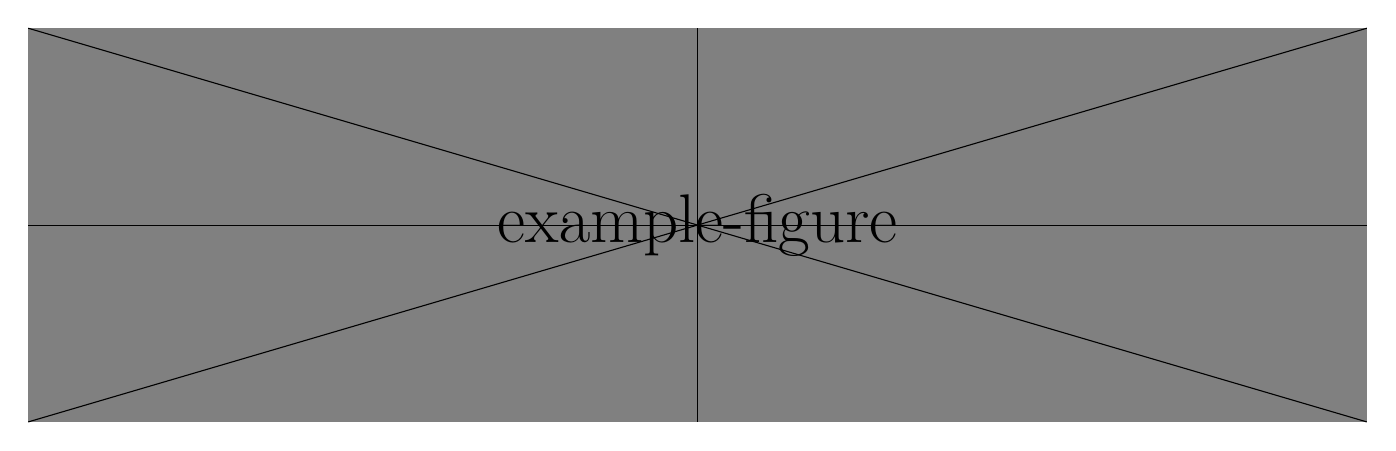
\begin{tikzpicture}
    % 绘制方框
    \fill[gray] (0, 0) rectangle (\sizeX, \sizeY); 
    % 绘制黑色对角线
    \draw[black] (0, 0) -- (\sizeX, \sizeY);       
    \draw[black] (0, \sizeY) -- (\sizeX, 0);       
    % 绘制黑色水平和垂直线
    \draw[black] (0, 0.5*\sizeY) -- (\sizeX, 0.5*\sizeY);       
    \draw[black] (0.5*\sizeX, 0) -- (0.5*\sizeX, \sizeY);       
    % 在中间放置字母
    \node at (0.5*\sizeX, 0.5*\sizeY) {\Huge example-figure};           
\end{tikzpicture}

\end{document}
